
\subsection{Carbon Number of \ce{O_x} Producing Degradation Products} \label{ss:c_number} %comparison by carbon number breakdown

\begin{figure}
    \begin{center}
        \includegraphics[width=\textwidth]{img/pentane_carbon_breakdown}
    \end{center}
    \caption{\ce{O_x} production attributed to carbon number of degradation products during pentane degradation in (a) MCM v3.2, (b) MCM v3.1, (c) CRI v2, (d) RADM2, (e) RACM, (f) RACM2, (g) MOZART-4, (h) CBM-IV and (i) CB05.}
    \label{f:pentane_carbon}
\end{figure}

\begin{figure}
    \begin{center}
        \includegraphics[width=\textwidth]{img/toluene_carbon_breakdown}
    \end{center}
    \caption{\ce{O_x} production distributed by carbon number of degradation products during toluene degradation in (a) MCM v3.2, (b) MCM v3.1, (c) CRI v2, (d) MOZART-4, (e) RADM2, (f) RACM, (g) RACM2, (h) CBM-IV and (i) CB05. In RACM, net \ce{O_x} consumption on the first two days is obtained as shown in Figure \ref{f:TOL_MCM_RACM} and described in Section \ref{sss:RACM_aromatic}.}
    \label{f:toluene_carbon}
\end{figure}

The timing and amount of \ce{O_x} produced throughout NMVOC degradation depends on how quickly the final degradation products of \ce{CO2} and \ce{H2O} are reached \citep{Butler:2011}. 
The day-time \ce{O_x} production of pentane and toluene in all mechanisms is attributed to the number of carbon atoms of the degradation products in Figures \ref{f:pentane_carbon} and \ref{f:toluene_carbon} respectively. 
This allows comparison of how quickly the emitted NMVOC is broken down into smaller degradation products.

Figure \ref{f:pentane_carbon} indicates that \ce{O_x} production from degradation products having the same number of carbon atoms as the emitted NMVOC has a larger influence in the near-explicit mechanisms than reduced mechanisms. 
This is compensated by an increased amount of \ce{O_x} production from degradation products having two or less carbon atoms. 
Thus the emitted VOC is broken down into smaller degradation products quicker in reduced mechanisms and cannot produce similar amounts of \ce{O_x} to near-explicit mechanisms.

An extreme case is the toluene degradation in MOZART, CBM-IV and CB05 shown in Figure \ref{f:toluene_carbon}. 
Toluene is immediately broken down into degradation products having two or less carbon atoms. 
This results in much lower \ce{O_x} production and TOPP values than other reduced mechanisms. 

Toluene degradation in CRI v2 differs from all other mechanisms as it has maximum \ce{O_x} production on the second day. 
Larger \ce{O_x} production from species having carbon number three or less than in the MCM v3.2 is responsible. 
This increase originates from extra \ce{HO2} produced from the reaction of the carbonyl mechanism species CARB3 with OH. 
This is discussed further in the supplement to this paper. 
\citet{Jenkin:2008} also acknowledge that reducing the MCM v3.1 chemistry of monoalkyl-substituted benzenes, such as toluene, was the most challenging and the resulting reduced chemistry over-estimates the \ce{O3} mixing ratios.

RACM2 toluene degradation also reaches maximum \ce{O_x} production on the second day. 
\ce{O_x} production from degradation products of a similar or higher carbon number to toluene indicate that toluene is broken down at slower in RACM2 than in MCM v3.2.

\subsection{Radical Production and Consumption Budgets} \label{ss:radicals}

\ce{O_x} production is directly to the conversion of NO to \ce{NO2} by peroxy radicals. 
Moreover, in this study maximum \ce{O3} production was achieved by emitting the amount of NO required to balance the radical source at each time step. 
A radical family for each mechanism was used to investigate the processes affecting production and loss budgets. 
This radical family includes all radical species and species involved in quick production and consumption cycles, such as PAN species and \ce{HO2NO2}.

\begin{figure}
    \begin{center}
        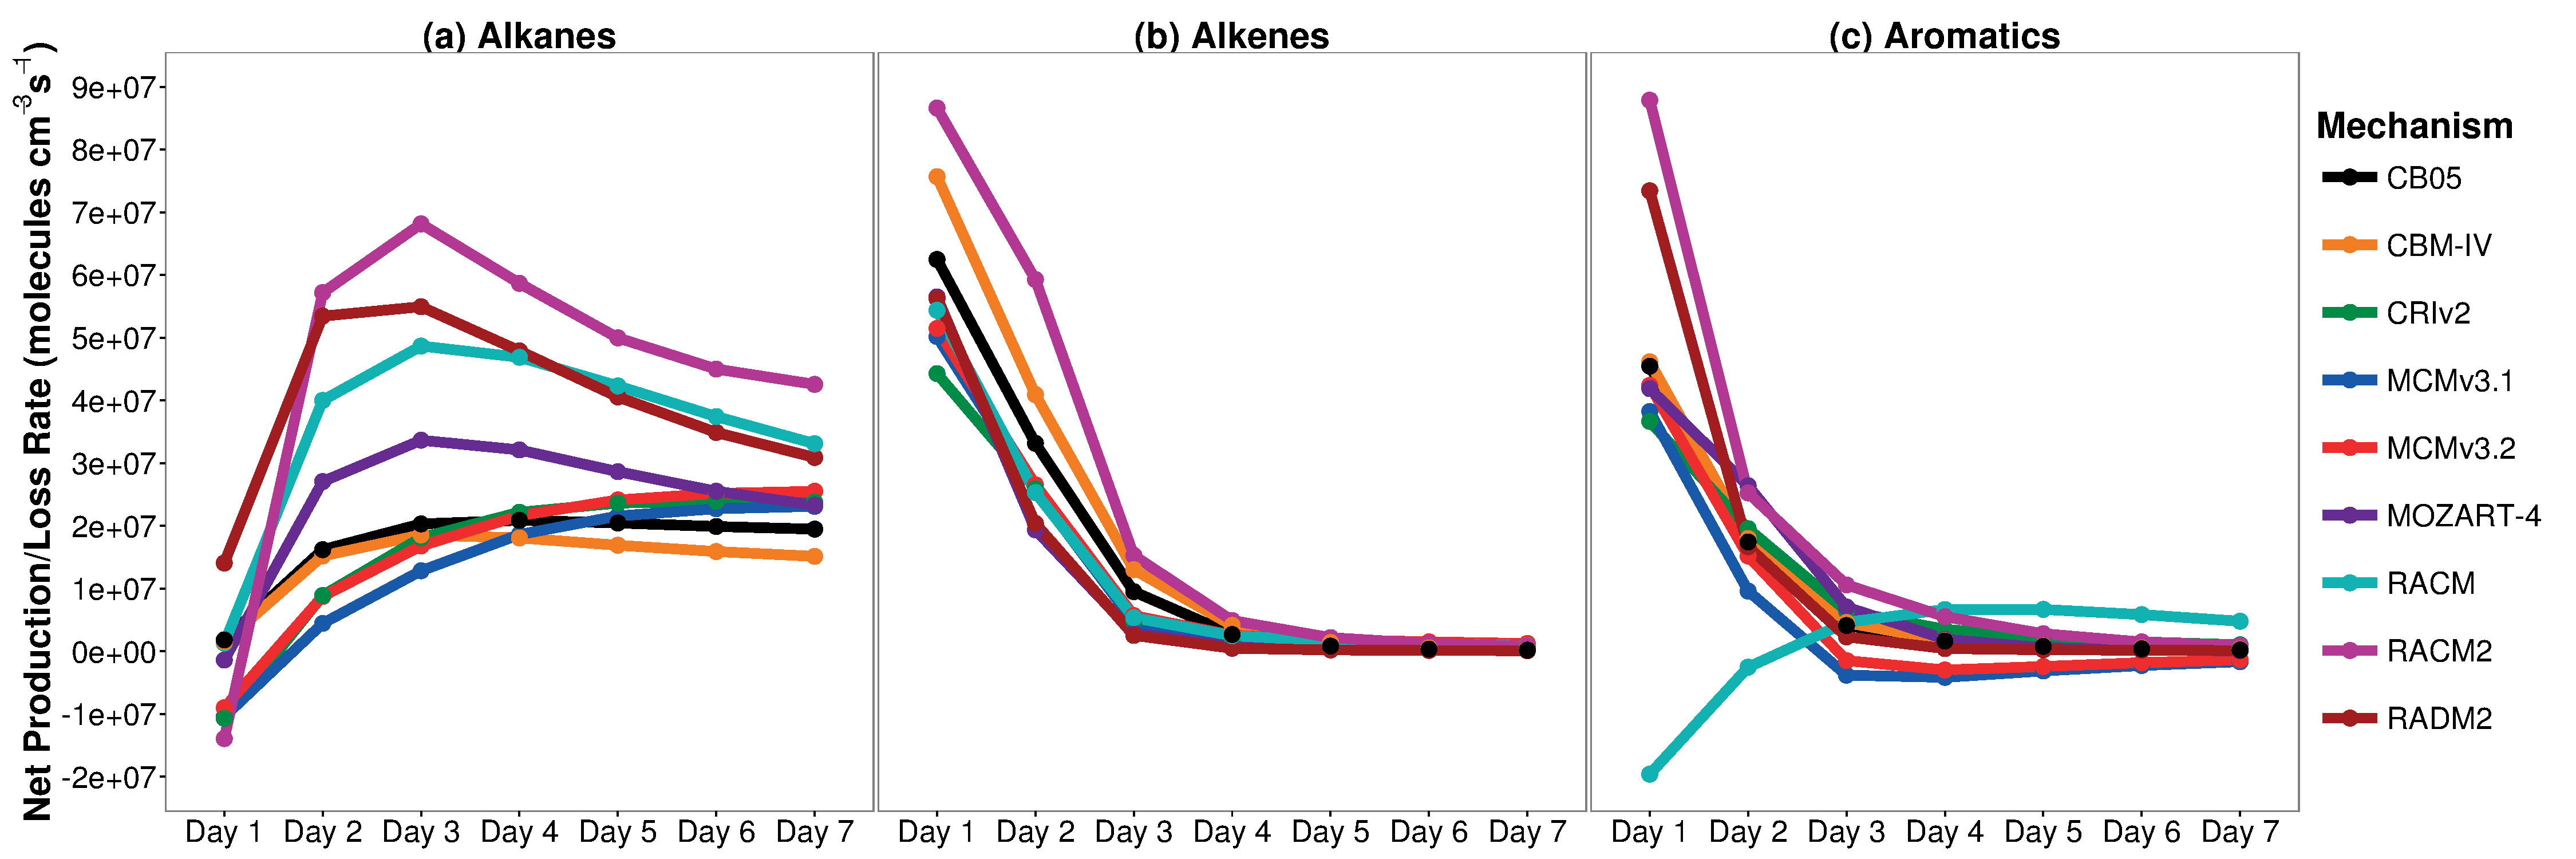
\includegraphics[width=\textwidth]{img/Net_radical_budgets}
    \end{center}
    \caption{The day-time net budget contribution of (a) alkane, (b) alkene and (c) aromatic degradation on the radical family in each mechanism.}
    \label{f:net_radical_budgets} 
\end{figure} 

\begin{figure}
    \begin{center}
        \includegraphics[width=\textwidth]{img/pentane_radical_budgets}
    \end{center}
    \caption{The processes influencing the radical family production and consumption budgets during pentane degradation are illustrated for (a) MCM v3.2, (b) MCM v3.1, (c) CRI v2, (d) RADM2, (e) RACM, (f) RACM2, (g) MOZART-4, (h) CBM-IV and (i) CB05.}
    \label{f:pentane_radical_budgets}
\end{figure}

\begin{figure}
    \begin{center}
        \includegraphics[width=\textwidth]{img/toluene_radical_budgets}
    \end{center}
    \caption{The processes influencing the radical family production and consumption budgets during toluene degradation is illustrated for (a) MCM v3.2, (b) MCM v3.1, (c) CRI v2, (d) RADM2, (e) RACM, (f) RACM2, (g) MOZART-4, (h) CBM-IV and (i) CB05.}
    \label{f:toluene_radical_budgets} 
\end{figure} 

The day-time net radical production and loss budgets due to alkane, alkene and aromatic degradation is shown in Figure \ref{f:net_radical_budgets}. 
The largest differences arise from alkane and aromatic degradation. 
Pentane and toluene radical budgets are attributed to the responsible processes in Figures \ref{f:pentane_radical_budgets} and \ref{f:toluene_radical_budgets} to determine the source of these differences.

In general, photolysis is the major radical production process and the reactions of radicals with other species, such as NO and \ce{HO2}, is the main radical sink. 
Reduced mechanisms include other processes to maintain radical production.

Figure \ref{f:pentane_radical_budgets} shows that initial VOC oxidation contributes to radical production in RADM2. 
This is represented by
\begin{reactionlist}
    \reactionitem{HC5 + OH}{HC5P + 0.25 XO2 + H2O}{new}{r:HC5_OH}
\end{reactionlist}
where HC5P is the pentyl peroxy radical and XO2 is an operator species which accounts for extra NO to \ce{NO2} conversions. 
XO2 is included in the radical family as it functions as a peroxy radical. 
This additional radical production pathway is responsible for the net first day radical production in RADM2.

The reactions of radicals lead to large net radical production in RACM after the first day. 
The main source being the reaction of HC5P with NO, 
\begin{center}
\refstepcounter{reaction}\label{r:HC5P_NO}
    \begin{tabular}{l@{\hskip 0.3cm}c@{\hskip 0.3cm}l@{\hskip 0.2cm}r}
        HC5P + NO & \reaction & 0.021 HCHO + 0.211 ALD + 0.722 KET & \reactionref{r:HC5P_NO} \\
        & & \hspace{2mm} + 0.599 HO2 + 0.031 MO2 + 0.245 ETHP & \\
        & & \hspace{2mm} + 0.334 XO2 + 0.124 ONIT + 0.876 NO2 &
    \end{tabular}
\end{center}
where HO2, MO2, ETHP and XO2 are the produced radical species. 
The larger net RADM2 and RACM radical production in Figure \ref{f:net_radical_budgets} is traced back to the extra radical production from reactions \reactionref{r:HC5_OH} and \reactionref{r:HC5P_NO} respectively.

Radical production in CBM-IV and CB05 is largely impacted by NMVOC initial oxidation and production from other radical reactions. 
Pentane degradation in these mechanisms is very similar and the CB05 reactions are considered here. 

Initial pentane degradation is via the PAR reaction with OH,
\begin{center}
\refstepcounter{reaction}\label{r:PAR_OH}
    \begin{tabular}{l@{\hskip 0.3cm}c@{\hskip 0.3cm}l@{\hskip 0.2cm}r}
        PAR + OH & \reaction & 0.87 XO2 + 0.13 XO2N + 0.11 HO2 + 0.06 ALD2 & \reactionref{r:PAR_OH} \\
        & & \hspace{2mm}  + 0.76 ROR + 0.05 ALDX - 0.11 PAR &
    \end{tabular}
\end{center}
where XO2, HO2 and ROR are the produced radical species. 
The mechanism species ROR decomposes immediately to either HO2 or \mbox{0.96 XO2 + 0.04 XO2N + 0.94 HO2 + 0.6 ALD2 + 0.02 ROR + 0.5 ALDX - 2.1 PAR}, once again XO2, HO2 and ROR are the produced radical species. 
The very fast decomposition of ROR and the use of XO2 to rapidly convert NO to \ce{NO2} leads to a rapid loss of radicals. 
The large production and consumption processes are balanced so that the net radical production correlates with that of the MCM v3.2.

The first day net radical production due to aromatic degradation are overestimated using RADM2 and RACM2 chemistry and underestimated in RACM. 
The RACM underestimation results from the degradation chemistry discussed in Section \ref{sss:RACM_aromatic}.

Figure \ref{f:toluene_radical_budgets} indicates that the RACM2 overestimation is due to radical production from reactions that do not involve radicals. 
The ozonolysis of the unsaturated dicarbonyl mechanism species DCB1 and DCB2 as well as the epoxy mechanism species EPX are additional reactions used to produce radicals.

The MCM v3.2 species TLEPOXMUC is analogous to EPX in RACM2. 
The ozonolysis rate constants are \mbox{$5 \times 10^{-18}$} and \mbox{$1 \times 10^{-16}$ cm$^3$ s$^{-1}$} respectively. 
The RACM2 rate constant is 20 times larger than that of the MCM v3.2 leading to excess radical production in RACM.

The ozonolysis of dicarbonyl species are included in RACM2 based on the recommendations of \citet{Bierbach:1994}. 
Dicarbonyl ozonolysis was not included in the MCM due to the uncertainties of these reactions \citep{Bloss:2005}.  
This additional radical source leads to larger net radical production.

\subsection{PAN Production and Consumption Budgets} \label{ss:PAN}

\begin{figure}
    \begin{center}
        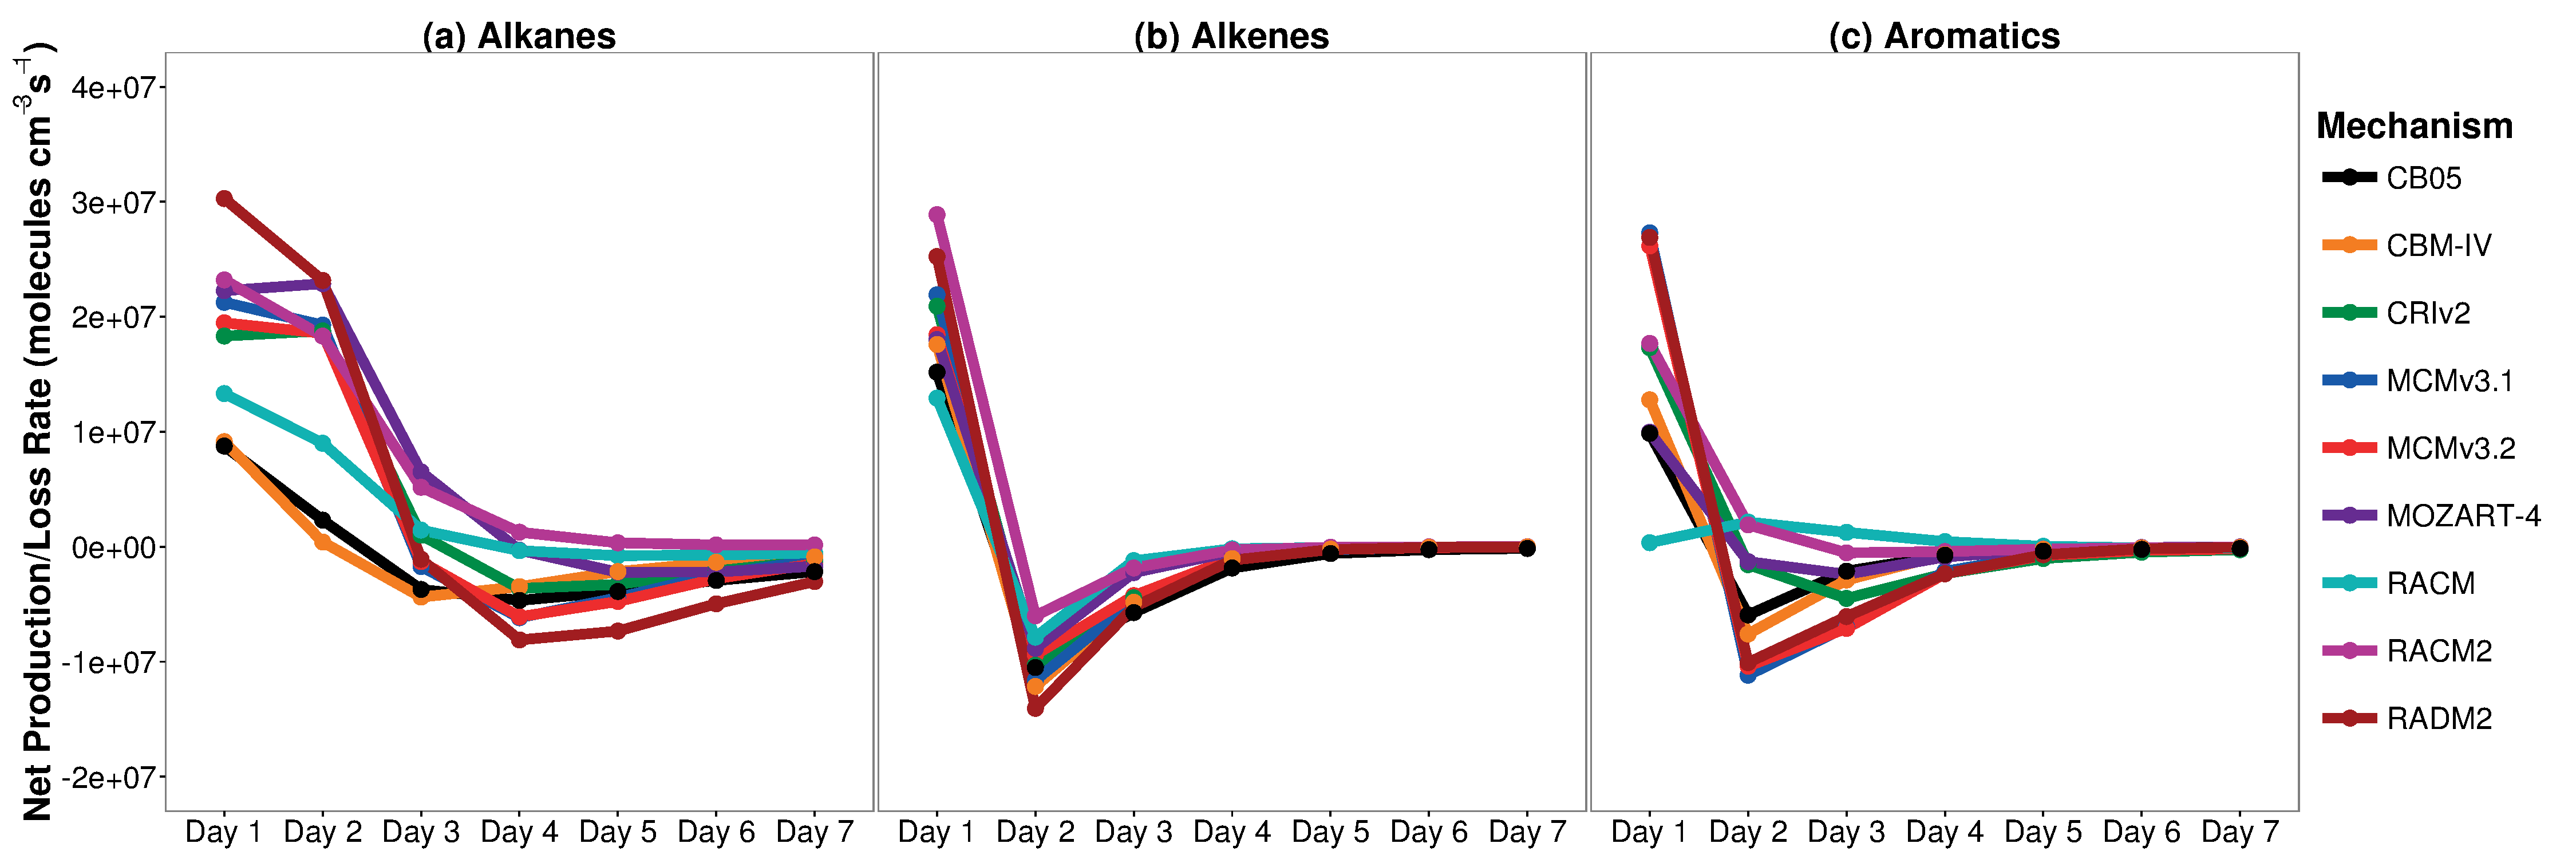
\includegraphics[width=\textwidth]{img/Net_PAN_budgets}
    \end{center}
    \caption{The day-time net budget contribution of (a) alkane, (b) alkene and (c) aromatic degradation on the PAN family in each mechanism.}
    \label{f:net_PAN}
\end{figure}

PAN chemistry influences \ce{O_x} production as it is both a radical and \ce{NO_x} sink \citep{Fischer:2014}. 
PAN production and consumption budgets were compared using a PAN family for each mechanism. 
This PAN family included all PAN species and associated acyl peroxy radicals.

\begin{figure}
    \begin{center}
        \includegraphics[width=\textwidth]{img/pentane_pan_budgets}
    \end{center}
    \caption{The processes influencing the PAN family production and loss budgets during pentane degradation are illustrated for (a) MCM v3.2, (b) MCM v3.1, (c) CRI v2, (d) RADM2, (e) RACM, (f) RACM2, (g) MOZART-4, (h) CBM-IV and (i) CB05.}
    \label{f:pentane_PAN}
\end{figure}

\begin{figure}
    \begin{center}
        \includegraphics[width=\textwidth]{img/toluene_pan_budgets}
    \end{center}
    \caption{The processes contributing to PAN family production and loss during toluene degradation are shown for (a) MCM v3.2, (b) MCM v3.1, (c) CRI v2, (d) RADM2, (e) RACM, (f) RACM2, (g) MOZART-4, (h) CBM-IV and (i) CB05.}
    \label{f:toluene_PAN}
\end{figure}

Figure \ref{f:net_PAN} shows the net day-time budgets of the PAN family from alkane, alkene and aromatic degradation. 
The PAN production and consumption budgets due to pentane and toluene degradation are expressed in terms of the contributing processes in Figures \ref{f:pentane_PAN} and \ref{f:toluene_PAN} respectively. 
Similar to the net radical budget analysis in Section \ref{ss:radicals}, the largest differences are from alkane and aromatics degradation.

Overall, reactions of aldehydes with OH are the main PAN family source with \reactionref{r:CH3CHO_OH} being the most prominent. 
The reaction of NO with acyl peroxy radicals is the major sink where \reactionref{r:CH3CO3_NO} is the main contributor. 
Other processes also impact production and consumption and these differ between mechanisms.
\begin{reactionlist}
    \reactionitem{\ce{CH3CHO + OH}}{\ce{CH3CO3 + H2O}}{new}{r:CH3CHO_OH}
    \reactionitem{\ce{CH3CO3 + NO}}{\ce{CH3O2 + NO2}}{new}{r:CH3CO3_NO}
\end{reactionlist}

PAN family production in both MCM mechanisms is further fuelled by alkoxy radical decomposition. 
This process is not included in any reduced mechanism and additional PAN family production is obtained through photolysis and reactions involving NO or \ce{O3}. 

CBM-IV and CB05 do not include any additional PAN family sources in alkane degradation. 
Whilst during aromatic degradation the additional PAN family source due to photolysis is minor. 
This results in lower net PAN family production compared to other mechanisms.

RADM2 has large net PAN family production regardless of the NMVOC type. 
The \reactionref{r:CH3CO3_NO} rate constant is $\sim$ 60\% slower than that of the MCM v3.2 rate constant resulting in less PAN family consumption. 
This rate constant was updated in RACM whilst the rate constant of \reactionref{r:CH3CHO_OH} was not significantly changed. 
This leads to more PAN family consumption in RACM and lower net PAN family production.

The detailed aromatic degradation chemistry of the MCM mechanisms produces the largest net PAN family production. 
The main sources of PAN family in the MCM are methyl glyoxal photolysis \reactionref{r:MGLYOX_hv} and reaction with OH \reactionref{r:MGLYOX_OH}.
\begin{reactionlist}
    \reactionitem{\ce{MGLYOX + h$\nu$}}{\ce{CH3CO3 + CO + HO2}}{new}{r:MGLYOX_hv}
    \reactionitem[\ce{O2}]{\ce{MGLYOX + OH}}{\ce{CH3CO3 + CO + H2O}}{new}{r:MGLYOX_OH}
\end{reactionlist}
In RADM2 and MOZART-4, \reactionref{r:MGLYOX_hv} and \reactionref{r:MGLYOX_OH} are also the main PAN family production sources. 
This contrasts to CRI v2 and RACM2 where these reactions are not as significant as PAN family production from \reactionref{r:CH3CHO_OH} and \reactionref{r:C2H5CHO_OH}.
\begin{reactionlist}
    \reactionitem{\ce{C2H5CHO + OH}}{\ce{C2H5CO3 + H2O}}{new}{r:C2H5CHO_OH}
\end{reactionlist}

The PAN family production budgets in CRI v2 and RACM2 in Figure \ref{f:toluene_PAN} peak on the second day rather than the first, similar to their \ce{O_x} production budgets in Figure \ref{f:toluene_carbon}. 
As outlined in Section \ref{ss:c_number}, CRI v2 toluene degradation has a larger contribution from degradation products with a carbon number three or less. 
This is reflected in CRI v2 PAN family production where the largest contributions are from reactions of \ce{CH3CHO} and \ce{C2H5CHO}.

The RACM2 ozonolysis reactions of unsaturated dicarbonyls are an additional PAN family source not included in other mechanisms. 
These reactions have a double contribution to PAN family production. 
Firstly, the mechanism acyl peroxy radical species RO3 is produced which sets off a reaction chain with \ce{CH3CHO}, represented as ALD in RACM2, being produced. 
These additional reactions result in a very different PAN family budget when compared to MCM v3.2.
